\documentclass[a4paper,14pt]{extarticle}
\usepackage[utf8]{inputenc}
\usepackage[english,russian]{babel}

\usepackage{amsthm}
\usepackage{graphicx}
\usepackage{caption}
\usepackage{amssymb}
\usepackage{amsmath}
\usepackage{mathrsfs}
\usepackage{euscript}
\usepackage{graphicx}
\usepackage{subfig}
\usepackage{caption}
\usepackage{color}
\usepackage{bm}
\usepackage{tabularx}
\usepackage{adjustbox}
\usepackage{float}
\usepackage{multirow}

\usepackage[toc,page]{appendix}

\usepackage{comment}
\usepackage{rotating}

\DeclareMathOperator*{\argmax}{arg\,max}
\DeclareMathOperator*{\argmin}{arg\,min}

\newtheorem{theorem}{Теорема}
\newtheorem{lemma}[theorem]{Лемма}
\newtheorem{definition}{Определение}[section]

\numberwithin{equation}{section}

\newcommand*{\No}{No.}

\begin{document}

% Титульный лист
%\input{./frontpage.tex}

% Аннотация
\newpage

\begin{abstract}

Исследуется проблема повышения качества моделей прогнозирования временных рядов на примере динамики курса акций. Рассматривается метод включения в модель внешних данных. Вводится предположение, что агрегированные знания опытных инвесторов повышают качество тестируемой модели. Рассматриваются нейросетевые методы машинного обучения и проводятся вычислительные эксперименты на реальных данных.

\smallskip

\textbf{Ключевые слова}: временные ряды, нейронные сети, краткосрочное прогнозирование

\end{abstract}


% Нумерация должна начинаться со второй страницы
\setcounter{page}{2}

% Оглавление
\newpage
\tableofcontents


% Введение
\newpage

\section{Введение}

\paragraph{Актуальность темы.} 
Предсказание цен на акций с помощью моделей машинного обучения является сложной задачей из-за высокой степени шума и множества факторов, влияющих на поведение цен.
В этом случае можно использовать перенос знаний с агрегированных ответов опытных инвесторов - \textit{модели автоследования} на \textit{базовую модель} предсказания.

\paragraph{Цель работы.} Одним из способов повышения качества алгоритма машинного обучения является использование дополнительных данных. Цель данной работы заключается
в повышении качества модели машинного обучения, предсказывающей временные ряды на примере курса акций. Для этого предлагается использовать передачу знаний от опытных инвесторов.

\paragraph{Новизна.}
Предложен подход, основанный на предположении о том, что внешние факторы, влияющие на курс акций, заложены в ответы опытных инвесторов.

\subsection{Обзор предметной области}

\begin{definition}
Модель автоследования --- агрегированные ответы опытных инвесторов о решении продажи или покупки акций, которые используются при обучении базовой модели.
\end{definition}

\begin{definition}
Базовая модель --- модель, при обучении которой используются ответы модели автоследования.
\end{definition}

\subsection{Предложенный метод}

Предлагается при обучении базовой модели использовать помимо данных временного ряда также ответы модели автоследования. Ожидается, что качество новых моделей будет превышать качество моделей, в обучении которых не использовались ответы модели автоследования.

В качестве экспериментальных данных используются реальные данные курса акций YNDX и ответы опытных инвесторов --- пользователей Тинькофф Инвестиций.

% Постановка
\newpage

\section{Постановка задачи}

Задан временной ряд 
$$x_{0}, x_{1}, x_{2}, ... x_{N}, \quad x_{i} \in \mathbb{R}^{6}$$
$$
    x_{i} &= 
    \begin{bmatrix}
        c_{i} & o_{i} & h_{i} & l_{i} & a_{i}
    \end{bmatrix}^{T},
$$
где \\
$c_{i}$ - цена закрытия, \\
$o_{i}$ - цена открытия, \\
$h_{i}$ - максимальная цена, \\
$l_{i}$ - минимальная цена, \\
$a_{i}$ - ответ модели автоследования ($a_{i} = 0$ в базовом варианте обучения модели)

\subsection{Постановка задача прогнозирования}

Требуется получить модель временного ряда:
$$\hat{c}_{t+k}(\mathbf{w}) = f_{t,k}(x_{t-M}, ..., x_{t}; \mathbf{w})$$
$$k = 1, ..., K,$$
где  \\
$K$ - горизонт прогнозирования, \\
$M$ - количество предыдущих наблюдений, \\
$\mathbf{w}$ - вектор параметров модели.

С помощью скользящего окна составлена выборка $\mathfrak{D}=(\mathbf{X},\mathbf{Y})$:

\begin{figure}[h!t]\center
{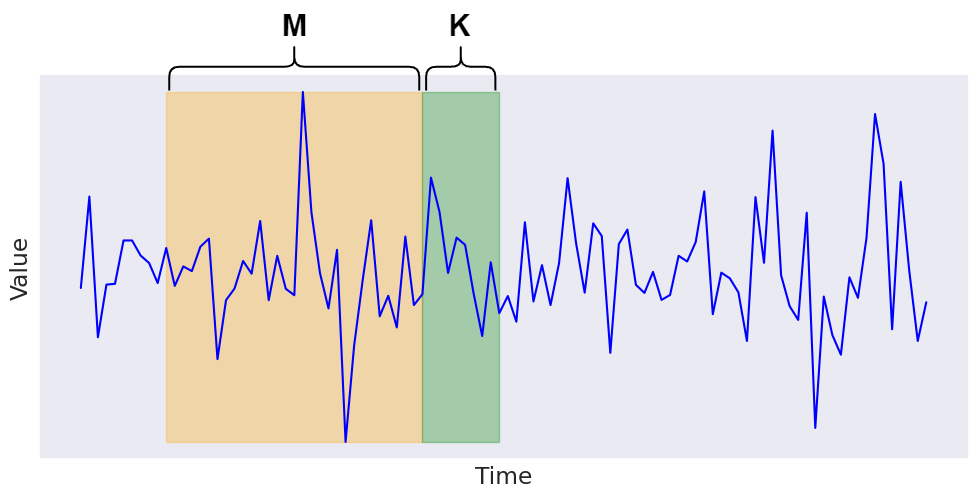
\includegraphics[width=0.8\textwidth]{results/slidingwindow.png}}
\caption{Использование скользящего окна для составления выборки}
\end{figure}

$
\mathbf{X} = \begin{pmatrix}
x_{0} & x_{1} & x_{2} & ... & x_{M}\\
x_{1} & x_{2} & x_{3} & ... & x_{M+1} \\
x_{2} & x_{3} & x_{4} & ... & x_{M+2} \\
\vdots & \vdots & \vdots & \vdots & \vdots \\
x_{N-K-M} & x_{N-K-M+1} & x_{N-K-M+2} & ... & x_{N-K} \\
\end{pmatrix} 

\mathbf{Y} = \begin{pmatrix}
c_{M+1} & c_{M+2} & c_{M+3} & ... & c_{M+K}\\
c_{M+2} & c_{M+3} & c_{M+4} & ... & c_{M+K+1} \\
c_{M+3} & c_{M+4} & c_{M+5} & ... & c_{M+K+2} \\
\vdots & \vdots & \vdots & \vdots & \vdots \\
c_{N-K+1} & c_{N-K+2} & c_{N-K+3} & ... & c_{N} \\
\end{pmatrix}
$

Функция потерь $\mathcal{L}$, используемая при обучении модели:
\[
\begin{aligned}
    \mathcal{L}(\mathbf{w,X,Y}) =& \sum\limits_{i=1}^{m}(f_{t,k}(x_{t-M}, ..., x_{t}; \mathbf{w})-c_{t+k}),
\end{aligned}
\]

Получаем оптимизационную задачу:
$$\hat{\mathbf{w}} = \arg\min_{\mathbf{w} \in \mathbb{W}} \mathcal{L}(\mathbf{w,X,Y,f}).$$

% Данные
\newpage

\section{Экспериментальные данные}

Эксперимент проводится для данных курса акций YNDX.

Задается временной ряд 
$$x_{1}, x_{2}, x_{3}, ..., x_{N}, \quad x_{i} \in \mathbb{R}^{5}$$
$$
    x_{i} = 
    \begin{bmatrix}
        c_{i} & o_{i} & h_{i} & l_{i} & a_{i}
    \end{bmatrix}^{T},
$$
где \\
$c_{i}$ - цена закрытия, \\
$o_{i}$ - цена открытия, \\
$h_{i}$ - максимальная цена, \\
$l_{i}$ - минимальная цена, \\
$a_{i}$ - ответ модели автоследования ($a_{i} = 0$ в базовом варианте обучения модели)

\subsection{Стационарность}

Исходный ряд приводится к стационарному виду следующими преобразованиями: \\
1) Дифференцирование: $y'_{t} = y_{t} - y_{t-1}$ \\ 
2) Сезонное дифференцирование $y''_{t} = y'_{t} - y'_{t-s}, \ s=5$ \\

Т.к. торги открыты только в будние дни, то выбранная длина сезона $s=5$.

\begin{figure}[h!t]\center
\subfloat[]
{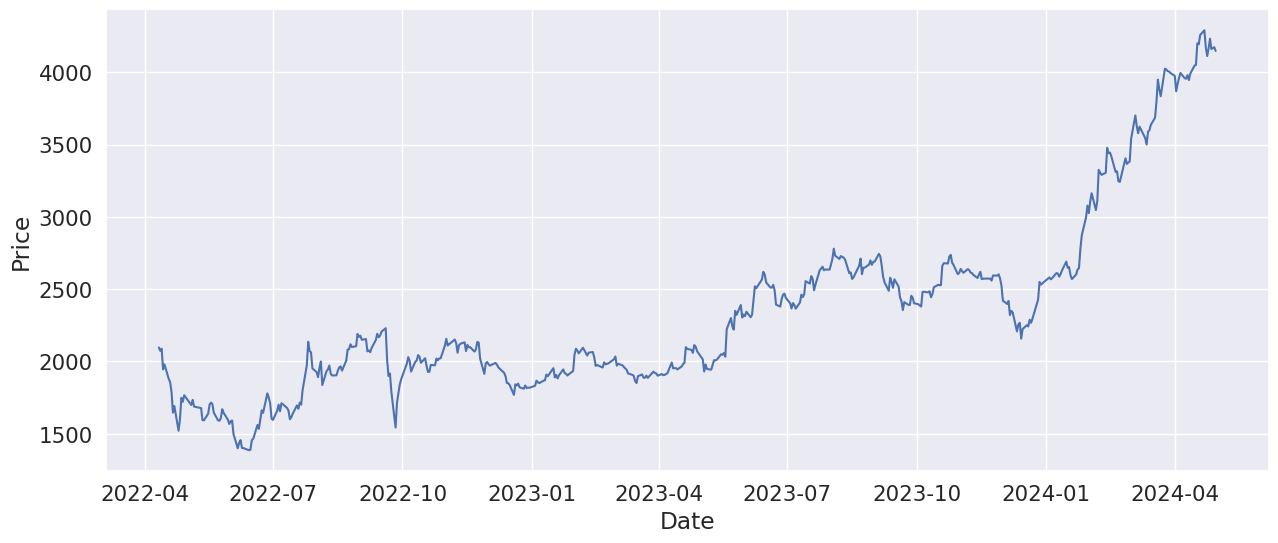
\includegraphics[width=0.5\textwidth]{results/yndx.png}}
\subfloat[]
{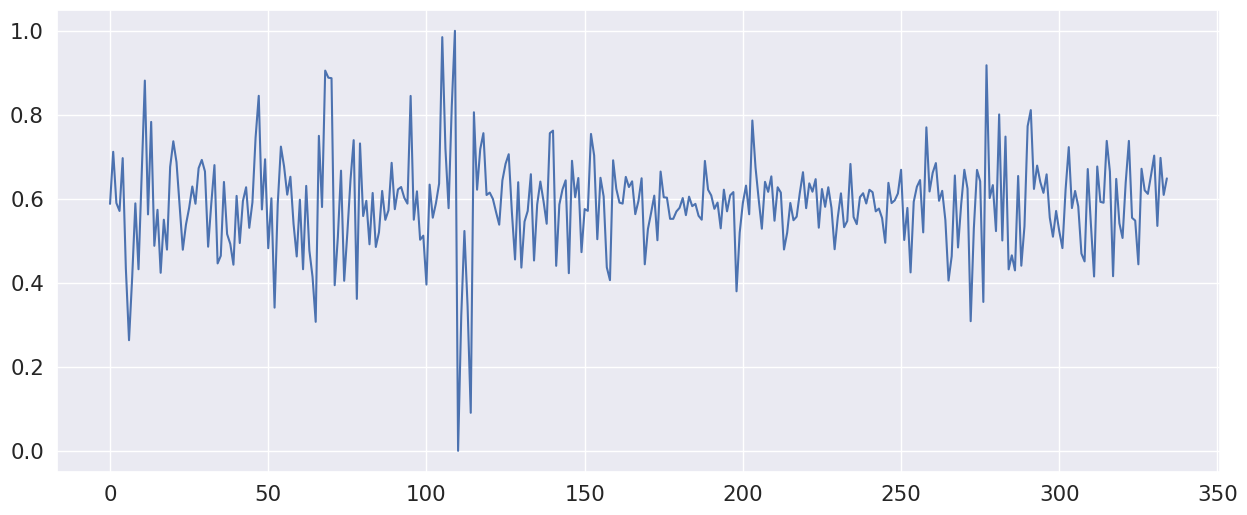
\includegraphics[width=0.5\textwidth]{results/yndx_stationary.png}}
\caption{Временной ряд курса акций YNDX до и после преобразований}
\end{figure}

Для проверки ряда на стационарность используется критерий KPSS~\cite{Критерии стационарности 1, Критерии стационарности 2}: \\
Для полученного ряда $p-value > 0.01$ \\
Для исходного ряда $p-value < 0.01$ 

Для визуальной оценки стационарности ряда также построим Q-Q plot:

\begin{figure}[h!t]\center
{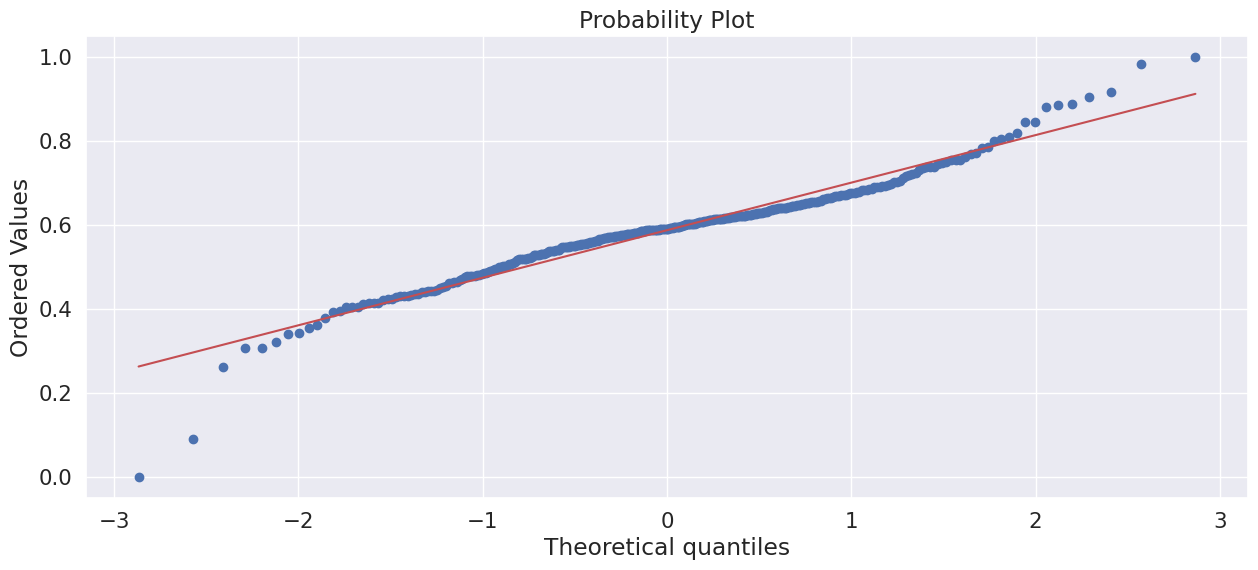
\includegraphics[width=0.8\textwidth]{results/qqplot.png}}
\caption{Q-Q plot полученного ряда}
\end{figure}

Видно, что точки на графике примерно лежат на прямой линии, следовательно распределение полученного временного ряда близко к нормальному.

Также воспользуемся анализом автокорреляционной функции:

\begin{figure}[h!t]\center
{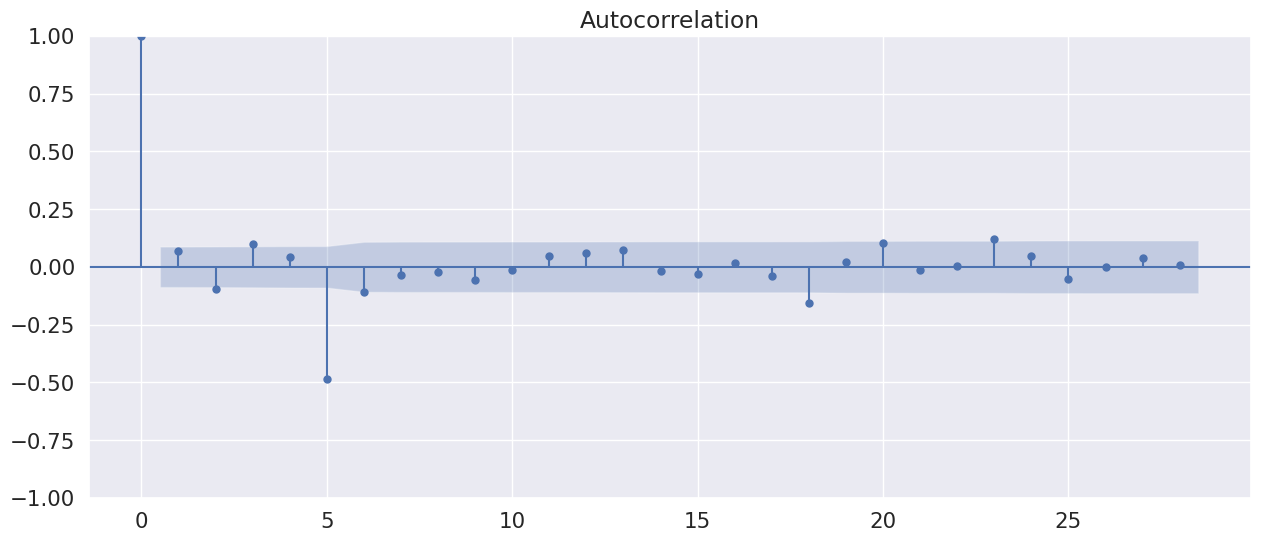
\includegraphics[width=0.8\textwidth]{results/acf.png}}
\caption{ACF полученного ряда}
\end{figure}

Близкие к нулю значения автокорреляций также указывают на стационарность полученного ряда.

\subsection{Составление выборки}

Методом скользящего окна составляется выборка $\mathfrak{D}=(\mathbf{X},\mathbf{Y})$:

\begin{figure}[h!t]\center
{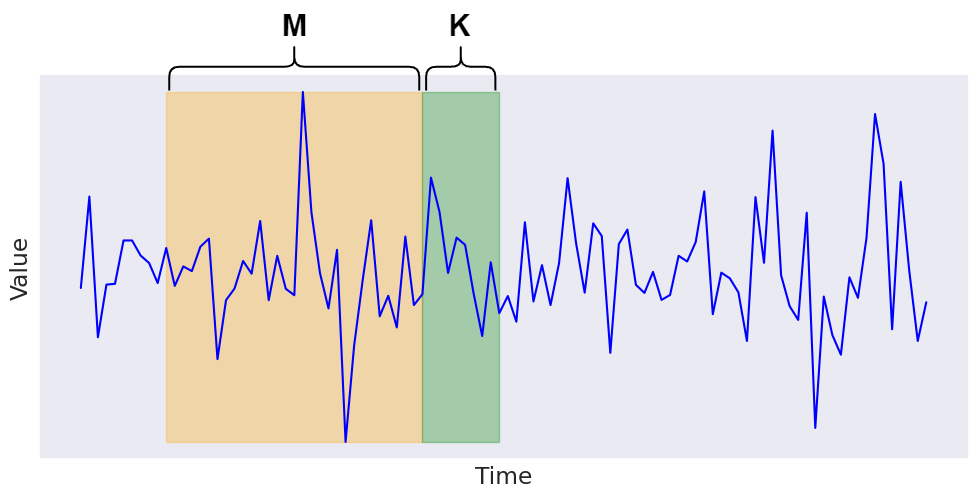
\includegraphics[width=0.8\textwidth]{results/slidingwindow.png}}
\caption{Метод скользящего окна}
\end{figure}

\small
\[
\mathbf{X} = 
\begin{pmatrix}
x_{1} & x_{2} & ... & x_{M}\\
x_{2} & x_{3} & ... & x_{M+1} \\
x_{3} & x_{4} & ... & x_{M+2} \\
\vdots & \vdots & \vdots & \vdots \\
x_{N-K-M+1} & x_{N-K-M+2} & ... & x_{N-K} \\
\end{pmatrix},
\mathbf{Y} = \begin{pmatrix}
c_{M+1} & c_{M+2} & ... & c_{M+K}\\
c_{M+2} & c_{M+3} & ... & c_{M+K+1} \\
c_{M+3} & c_{M+4} & ... & c_{M+K+2} \\
\vdots & \vdots & \vdots & \vdots \\
c_{N-K+1} & c_{N-K+2} & ... & c_{N} \\
\end{pmatrix},
\]
\normalsize

где  $M$ - размер окна, $K$ - горизонт прогнозирования.

\bigskip

В качестве целевых значений используется цена закрытия.

\bigskip

В соотношении 80/20 выборка делится на обучающую и тестовую части: YNDX-train, YNDX-test.

% Эксперимент
\newpage

\section{Вычислительный эксперимент}

\subsection{Модель автоследования} 

Автоследование --- способ инвестирования, при котором все желающие могут подключиться к стратегии более опытного инвестора (он же автор стратегии) и автоматически повторять все его сделки на своем счете. 

Для создания модели автоследования выделяются инвесторы - авторы стратегий автоследования Тинькофф инвестиций. 
\[\text{Ответ инвестора} = \frac{\text{Сумма сделки}}{\text{Объем портфеля}}\]

Путем усреднения ответов инвесторов о продаже или покупке акций составляется временной ряд $a_{0}, ..., a_{N}, a_{i} \in [-1, 1]$.

\begin{figure}[h!t]\center
{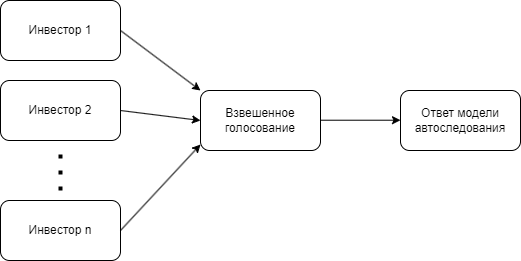
\includegraphics[width=0.8\textwidth]{results/voting.png}}
\caption{Модель автоследования}
\end{figure}

\subsection{Подготовка данных} 
Эксперимент проводится для временного ряда курса акций YNDX. 

Ряд приводится к стационарному виду следующими преобразованиями: \\
1) Дифференцирование: $y'_{t} = y_{t} - y_{t-1}$ \\ 
2) Сезонное дифференцирование $y' '_{t} = y'_{t} - y'_{t-s}, \ s=5$ \\

\begin{figure}[h!t]\center
\subfloat[]
{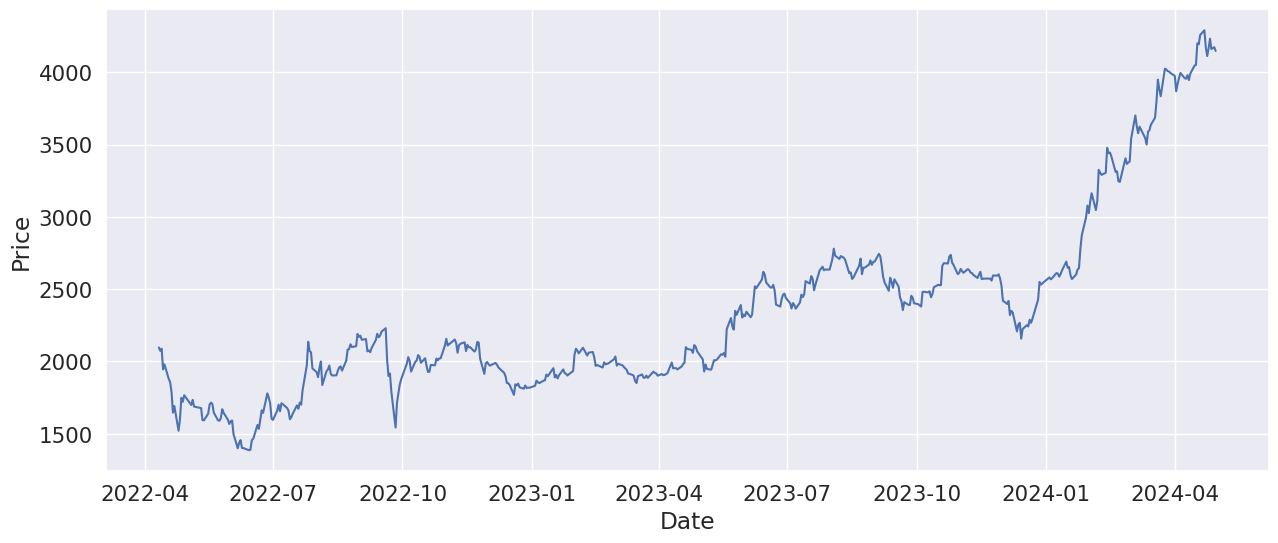
\includegraphics[width=0.5\textwidth]{results/yndx.png}}
\subfloat[]
{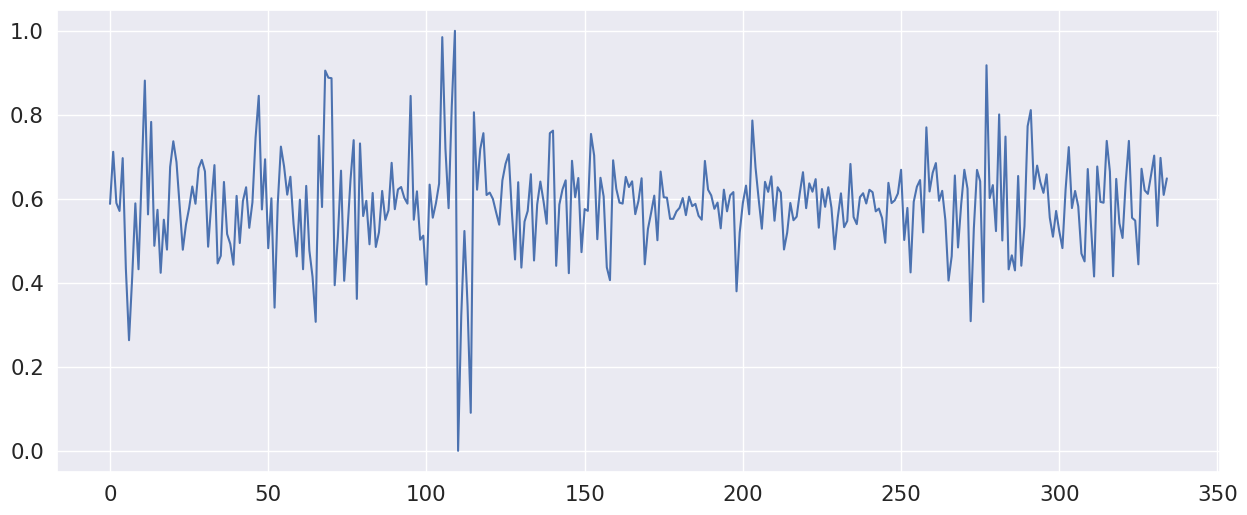
\includegraphics[width=0.5\textwidth]{results/yndx_stationary.png}}\\
\caption{Временной ряд курса акций YNDX до и после преобразований}
\end{figure}

Для проверки ряда на стационарность используется критерий KPSS: \\
Для исходного ряда $p-value < 0.01$ \\
Для полученного ряда $p-value > 0.01$ \\

\begin{figure}[h!t]\center
{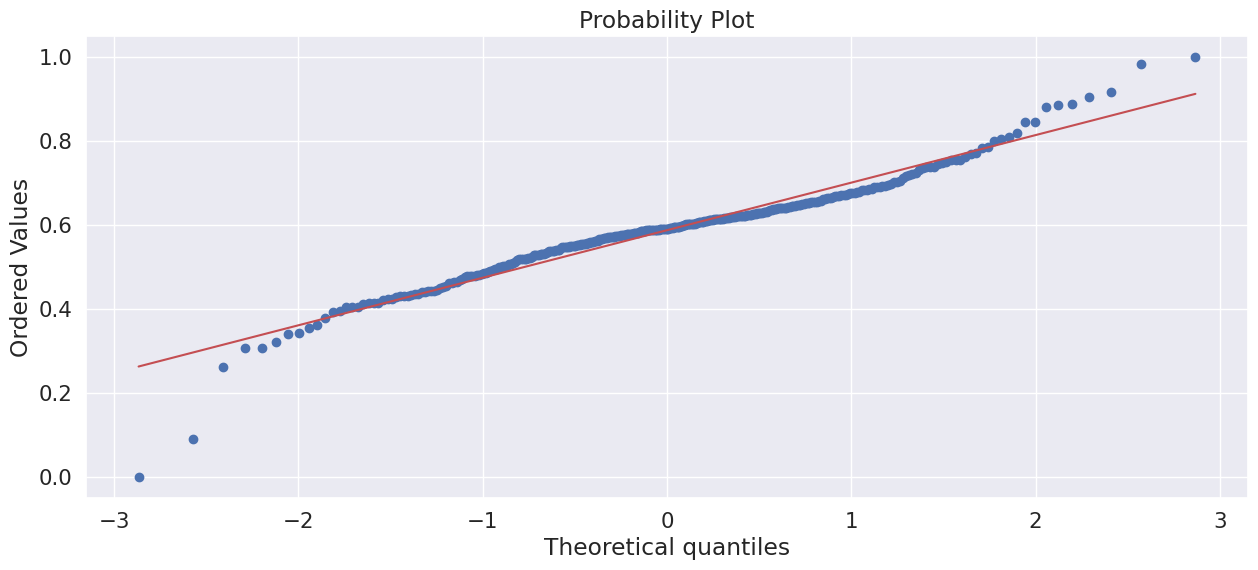
\includegraphics[width=0.8\textwidth]{results/qqplot.png}}
\caption{Q-Q plot полученного ряда}
\end{figure}

\begin{figure}[h!t]\center
{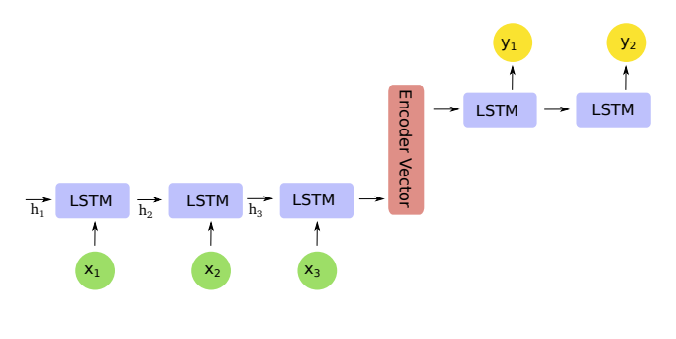
\includegraphics[width=0.8\textwidth]{results/seq2seq.png}}
\caption{sequence-to-sequence архитектура}
\end{figure}

\begin{table}[h!t]
\begin{center}
\caption{Выборки}
\label{table_2}
\begin{tabular}{|c|c|}
\hline
	Выборка & Пояснение \\
	\hline
	\multicolumn{1}{|l|}{YNDX-Train}
	& Обучающая часть \\
	\hline
	\multicolumn{1}{|l|}{YNDX-Test}
	& Тестовая часть \\
	\hline
	\multicolumn{1}{|l|}{TMOS-Train}
	& Обучающая часть \\
	\hline
	\multicolumn{1}{|l|}{TMOS-Test}
	& Тестовая часть \\
\hline

\end{tabular}
\end{center}
\end{table}


\subsection{Нахождение оптимального размера окна}

Для формирования обучающей выборки используется метод скользящего окна. 
Сравнение качества базовой модели на тестовой выборке в завимости от размера окна.


\subsection{Анализ качества модели прогнозирования}

В качестве базовой модели для задачи прогнозирования используется seq2seq архитектура на основе LSTM модели. При этом метод пресказания - рекурсивный.

Сравнение качества базовой модели на тестовой выборке в зависимости от использования ответов модели автоследования.

\begin{figure}[h!t]\center
{\includegraphics[width=0.8\textwidth]{results/loss_forecasting.png}}
\caption{Качество прогнозирования на тестовой выборке. Все результаты усреднены по 5 запускам}
\end{figure}

На рис. показан график зависимости средней кварадтичной ошибки на отложенной тестовой выборке между истинными значениями ряда и ответами модели.

\begin{figure}[h!t]\center
\subfloat[]
{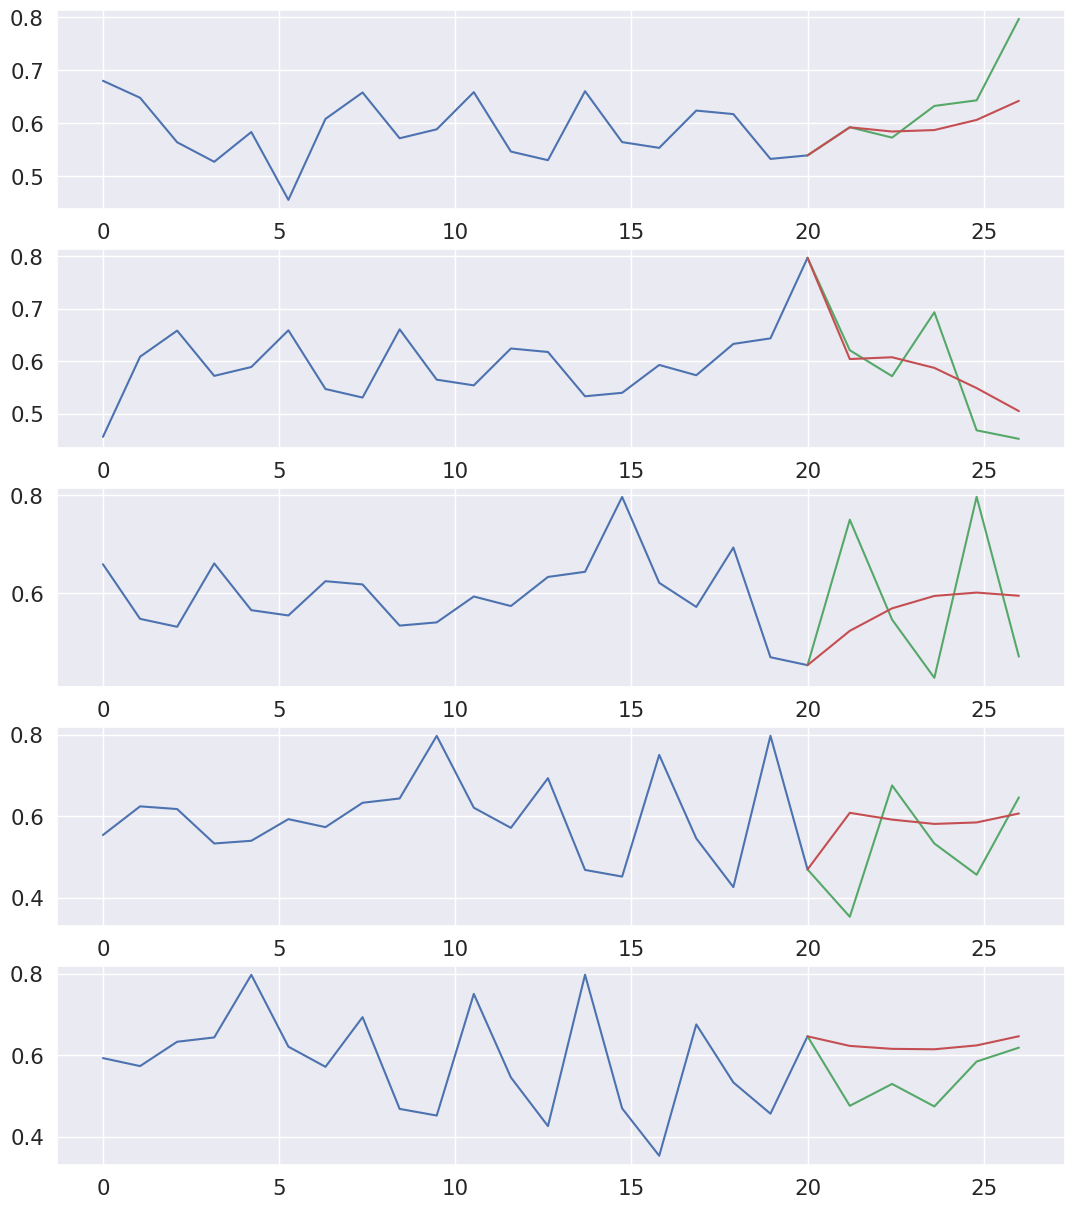
\includegraphics[width=0.5\textwidth]{results/forecasting_example_base.png}}
\subfloat[]
{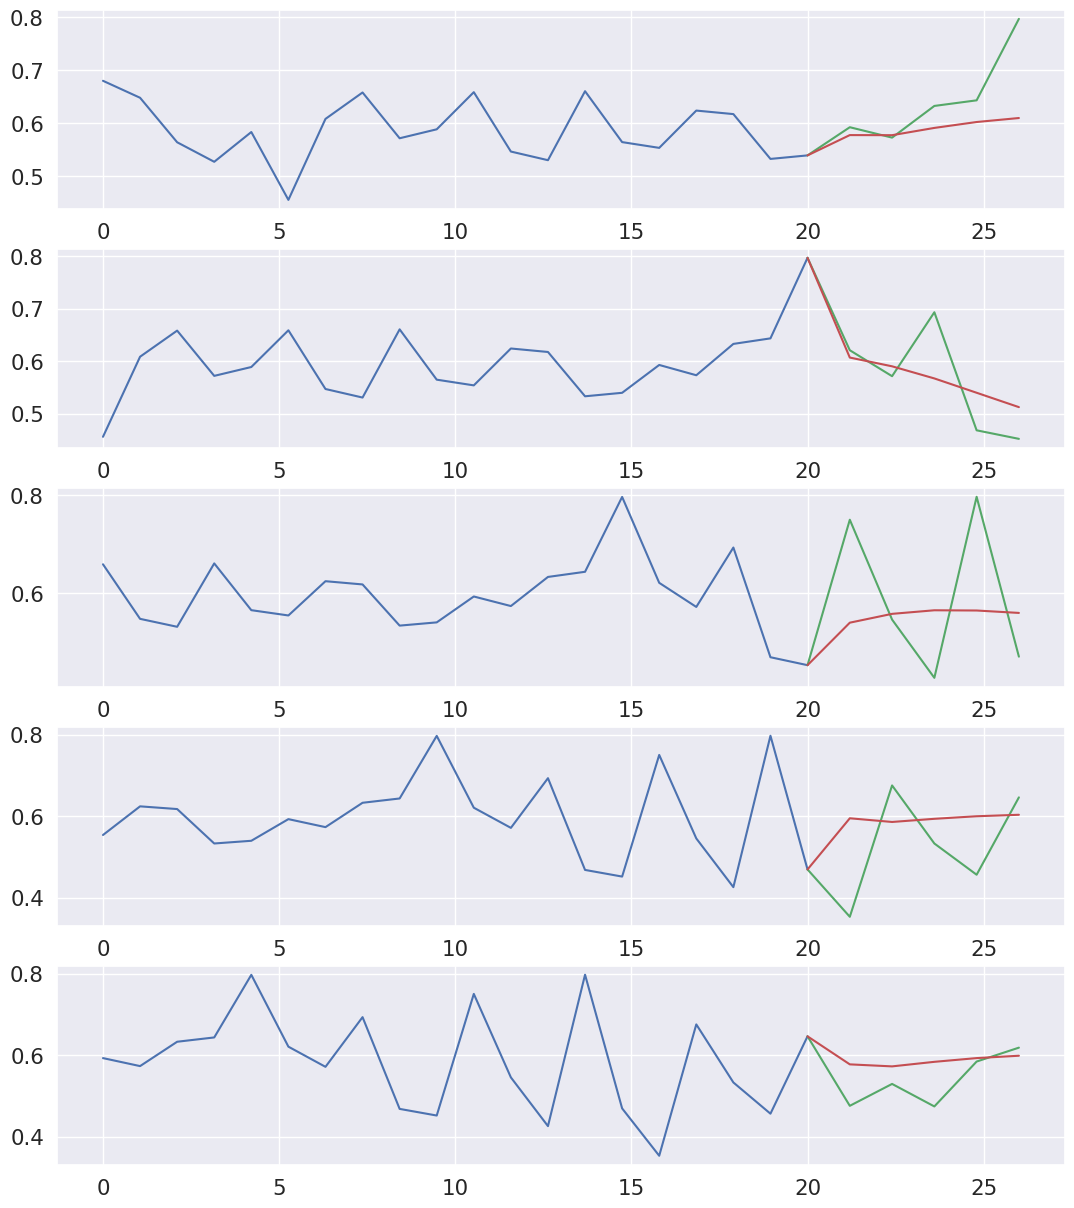
\includegraphics[width=0.5\textwidth]{results/forecasting_example_auto.png}}\\
\caption{Сравнение результатов прогнозирования. a) Без использования модели автоследования; b) С использованием модели автоследования}
\end{figure}

На рис. показаны примеры прогнозирования базовой модели на отложенной тесовой выборке.

На графиках видно, что модель, использующая ответы модели автоследования, показывает лучшее качество прогнозирования, при этом наблюдается снижение средней квадратичной ошибки. 

\subsection{Код вычислительного эксперимента}

Весь код вычислительного эксперимента представлен в~\cite{Github}. Также доступны письменный отчет и результаты экспериментов.

% Заключение
\newpage

\section{Заключение}

\begin{table}[h!t]
\begin{center}
\caption{Результаты экспериментов}
\label{final_results}
\resizebox{\linewidth}{!}{
\begin{tabular}{|c|c|c|c|c|}
\hline
\textbf{Выборка} & \textbf{Модель} & \textbf{\begin{tabular}[c]{@{}c@{}}Дополнительные\\ данные\end{tabular}} & \textbf{\begin{tabular}[c]{@{}c@{}}Корреляция\\ Пирсона\end{tabular}} & \textbf{MSE} \\
\hline
\hline
& ARIMA & & $0{,}340$ & $0{,}0183$ \\
\hline
\hline
\multirow{4}{*}{YNDX-Train5} & \multicolumn{1}{|c|}{\multirow{2}{*}{Seq2Seq LSTM}} & --- & $0{,}476 \pm 0{,}027$ & $0{,}0175 \pm 0{,}0003$ \\ \cline{3-3} \cline{4-4} \cline{5-5}
                            & \multicolumn{1}{|c|}{}                                    & Автоследование & $0{,}510 \pm 0{,}036$ & $0{,}0171 \pm 0{,}0001$ \\ 
                            \cline{2-3} \cline{4-4} \cline{5-5}
                            & \multicolumn{1}{|c|}{\multirow{2}{*}{Seq2Seq Transformer}} & --- & $0{,}379 \pm 0{,}039$ & $0{,}0225 \pm 0{,}0005$ \\ 
                            \cline{3-3} \cline{4-4} \cline{5-5}
                            & \multicolumn{1}{|c|}{}                                    & Автоследование & $0{,}401 \pm 0{,}035$ & $0{,}0219 \pm 0{,}0004$ \\ 
\hline
\hline
\multirow{4}{*}{YNDX-Train15} & \multicolumn{1}{|c|}{\multirow{2}{*}{Seq2Seq LSTM}} & --- & $0{,}553 \pm 0{,}004$ & $0{,}0186 \pm 0{,}0008$ \\ \cline{3-3} \cline{4-4} \cline{5-5}
                            & \multicolumn{1}{|c|}{}                                    & Автоследование & $0{,}599 \pm 0{,}006$ & $0{,}0175 \pm 0.0007$ \\ 
                            \cline{2-3} \cline{4-4} \cline{5-5}
                            & \multicolumn{1}{|c|}{\multirow{2}{*}{Seq2Seq Transformer}} & --- & $0{,}415 \pm 0{,}010$ & $0{,}0229 \pm 0{,}0006$ \\ 
                            \cline{3-3} \cline{4-4} \cline{5-5}
                            & \multicolumn{1}{|c|}{}                                    & Автоследование & $0{,}440 \pm 0{,}001$ & $0{,}0218 \pm 0{,}0009$ \\
\hline
\hline
\multirow{4}{*}{YNDX-Train30} & \multicolumn{1}{|c|}{\multirow{2}{*}{Seq2Seq LSTM}} & --- & $0{,}478 \pm 0{,}006$ & $0{,}0195 \pm 0{,}0005$ \\ \cline{3-3} \cline{4-4} \cline{5-5}
                            & \multicolumn{1}{|c|}{}                                    & Автоследование & $0{,}538 \pm 0{,}007$ & $0{,}0186 \pm 0{,}0017$ \\ 
                            \cline{2-3} \cline{4-4} \cline{5-5}
                            & \multicolumn{1}{|c|}{\multirow{2}{*}{Seq2Seq Transformer}} & --- & $0{,}406 \pm 0{,}011$ & $0{,}0211 \pm 0{,}0010$ \\ 
                            \cline{3-3} \cline{4-4} \cline{5-5}
                            & \multicolumn{1}{|c|}{}                                    & Автоследование & $0{,}425 \pm 0{,}009$ & $0{,}0210 \pm 0{,}0009$ \\
\hline
\end{tabular}
}
\end{center}
\end{table}


В работе рассмотрена проблема повышения качества моделей прогнозирования временных рядов на примере динамики курса акций. Рассмотрены методы прогнозирования на основе рекуррентных сетей и моделей трансформеров. Был предложен подход включения в модель дополнительных данных --- агрегированных знаний опытных инвесторов.

В ходе экспериментов, проведенных на реальных данных, было показано, что предложенный метод работает и повышает качество тестируемых моделей. Результаты экспериментов представлены в таблице~\ref{final_results}. 

Из таблицы видно, что качество модели зависит от размера входного окна: модели, обученные на выборке с входным окном размера 15, имеют наилучшее качество. Также во всех экспериментах качество тестируемой модели повышается при использовании дополнительных данных модели автоследования.

% Библиографические ссылки
\newpage

\begin{thebibliography}{99}

    \bibitem{ARIMA} 
    \textit{Лукашин Ю.П.} Адаптивные методы краткосрочного прогнозирования временных рядов. Финансы и статистика, 2003

    \bibitem{Stock price ARIMA}
    \textit{Ariyo A.A.,Adewumi A.O.} Stock price prediction using the ARIMA model, 2014

    \bibitem{Критерии стационарности 1}
    \textit{Patterson K.} Unit Root Tests In Time Series Volume 1, 2011

    \bibitem{Критерии стационарности 2}
    \textit{Herranz E.} Unit root tests, 2017

    \bibitem{LSTM1}
    \textit{Hochreiter S., Schmidhuber J.} Neural Computation 9(8), 1997

    \bibitem{LSTM2}
    \textit{Greff K., Schmidhuber J.} LSTM: A Search Space Odyssey, 2017

    \bibitem{LSTM3}
    \textit{Christopher Olah} Understanding LSTM Networks, 2015 \\
    https://colah.github.io/posts/2015-08-Understanding-LSTMs

    \bibitem{EncoderDecoder} 
    \textit{Cho K.} On the Properties of Neural Machine Translation: Encoder–Decoder Approaches, 2014

    \bibitem{RNN Attention}
    \textit{Bahdanau D.} Neural Machine Translation By Jointly Learning To Align And Translate, 2016

    \bibitem{Attention Mechanisms}
    \textit{Dichao Hu} An Introductory Survey on Attention Mechanisms in NLP Problems, 2018

    \bibitem{Self-Attention}
    \textit{Lin Z., Bengio Y.} A Structured Self-Attentive Sentence Embedding, 2017

    \bibitem{Attention is all you need}
    \textit{Vaswani A. et al.} Attention Is All You Need, 2017

    \bibitem{Positional Encoding}
    \textit{Shaw P., Uszkoreit J., Vaswani A.} Self-Attention with Relative Position Representations, 2018

    \bibitem{Adam}
    \textit{Kingma D. P., Ba J.} Adam: A Method for Stochastic Optimization, 2017

    \bibitem{Transformer Time Series}
    \textit{Wu N., Green B.} Deep Transformer Models for Time Series Forecasting, 2020

    \bibitem{LogTrans}
    \textit{Li S., Jin X.} Enhancing the Locality and Breaking the Memory Bottleneck of Transformer on Time Series Forecasting, 2019

    \bibitem{Autoformer}
    \textit{Wu H., Xu J.} Autoformer: Decomposition transformers with auto-correlation for long-term series forecasting, 2021

    \bibitem{Informer}
    \textit{Zhou H., Zhang S.} Informer: Beyond efficient transformer for long sequence time-series forecasting, 2021

    \bibitem{Pyraformer}
    \textit{Liu S., Yu H.} Pyraformer: Low-complexity pyramidal attention for long-range time series modeling and forecasting, 2021

    \bibitem{FEDformer}
    \textit{Zhou T., Ma Z.} FEDformer: Frequency Enhanced Decomposed Transformer for Long-term Series Forecasting, 2022
    
    \bibitem{iTransformer}
    \textit{Liu Y., Hu T., Zhang H.} iTransformer: Inverted Transformers Are Effective for Time Series Forecasting, 2023

    \bibitem{Лекции}
    \textit{Воронцов К. В.} Машинное обучение, курс лекций
    
    \bibitem{Github}
    \textit{Отчет} https://github.com/kbayazitov/StockPricingForecasting
	
\end{thebibliography}


\end{document}